\documentclass[8pt, landscape, a4paper]{extarticle}

% --- 核心宏包 ---
\usepackage[UTF8]{ctex}
\usepackage[margin=0.8cm, top=1cm, bottom=1.3cm]{geometry}
\usepackage{multicol}
\usepackage{xcolor}
\usepackage{tcolorbox}
\usepackage{enumitem}
\usepackage{amsmath}
\usepackage{amssymb}
\usepackage{fontspec}
\usepackage{tikz}
\usetikzlibrary{arrows.meta, shapes}

% --- 去掉页码 ---
\pagestyle{empty}

% --- 颜色定义 (Dark Blue 主题) ---
\definecolor{headerblue}{RGB}{44, 62, 80}      % Midnight Blue
\definecolor{navcolor}{RGB}{211, 84, 0}        % 导航橙
\definecolor{intuitioncolor}{RGB}{41, 128, 185}% 直觉蓝
\definecolor{accentcolor}{RGB}{192, 57, 43}    % 强调红
\definecolor{section2}{RGB}{22, 160, 133}      % 绿色
\definecolor{dividergray}{RGB}{220, 220, 220}

% --- 全局设置 ---
\setlength{\parindent}{0pt}
\setlength{\columnsep}{0.4cm} 
\linespread{1.1} 

% --- 列表样式 ---
\setlist[itemize]{leftmargin=1.2em, nosep, itemsep=2pt, topsep=2pt, label=$\textcolor{headerblue}{\vcenter{\hbox{\tiny$\bullet$}}}$ }
\setlist[description]{leftmargin=0.2em, style=sameline, nosep, itemsep=2pt, font=\bfseries}

% --- Box 样式 ---
\newtcolorbox{mybox}[2][]{%
  colback=white,
  colframe=#2,
  coltitle=white,
  boxrule=1pt,             
  arc=2mm,                 
  left=4pt, right=4pt, top=3pt, bottom=3pt, 
  toptitle=3pt, bottomtitle=3pt, 
  fonttitle=\bfseries\sffamily\large,
  title={#1},
  after skip=5pt          
}

% --- 自定义命令 ---
\newcommand{\subt}[1]{{\vspace{2pt}\textbf{\large \textcolor{black}{#1}}}}

\newcommand{\boxdesc}[1]{%
    \textit{\small \textcolor{gray}{#1}}%
    \par\vspace{2pt}%
    {\color{dividergray}\hrule height 0.5pt}%
    \vspace{2pt}%
}

\newcommand{\sepline}{%
    \par \vspace{3pt}%
    {\color{dividergray}\hrule height 0.5pt}%
    \par \vspace{3pt}%
}

% 公式间距
\setlength{\abovedisplayskip}{3pt}
\setlength{\belowdisplayskip}{3pt}

\begin{document}

% --- 页眉 ---
\begin{center}
    {\Huge \textbf{\sffamily \textcolor{headerblue}{泛函分析 Functional Analysis Cheat Sheet}}} \\
    \vspace{0.2cm}
    {\large \texttt{Infinite Dimensional Linear Algebra: Spaces of Functions}}
\end{center}

% --- 开始四栏布局 ---
\begin{multicols*}{4}

% === 第一栏 ===

\begin{mybox}[️ 场景导航 (Use Cases)]{navcolor}
    \boxdesc{遇到什么问题 $\to$ 用什么工具}
    \begin{itemize}[itemsep=2pt]
        \item \textbf{量子力学} $\to$ 希尔伯特空间 / 算子谱
        \item \textbf{偏微分方程 (PDE)} $\to$ 索伯列夫空间 / 弱解
        \item \textbf{机器学习核方法} $\to$ RKHS (再生核希尔伯特空间)
        \item \textbf{信号压缩} $\to$ 巴拿赫空间 / 小波基
        \item \textbf{变分法} $\to$ 欧拉-拉格朗日方程
        \item \textbf{分布理论} $\to$ 广义函数 ($\delta$ 函数)
    \end{itemize}
\end{mybox}

\begin{mybox}[1. 空间层级 (Hierarchy)]{headerblue}
    \boxdesc{从松散到严格}
    
    \subt{1. 线性空间 (Vector Space)}
    只有加法和数乘。
    \sepline
    
    \subt{2. 赋范空间 (Normed Space)}
    有长度 $\|x\|$。
    \textbf{Banach 空间}: 完备的赋范空间 (柯西序列收敛)。
    \textit{例: $L^p$ 空间 ($p \neq 2$), $C[a,b]$。}
    \sepline
    
    \subt{3. 内积空间 (Inner Product)}
    有角度 $\langle x, y \rangle$。
    \textbf{Hilbert 空间}: 完备的内积空间。
    \textit{例: $L^2$ 空间, $\mathbb{R}^n$。}
    $$ \|x\| = \sqrt{\langle x, x \rangle} $$
\end{mybox}

\begin{mybox}[2. 核心不等式 (Inequalities)]{headerblue}
    \boxdesc{分析的武器}
    
    \subt{Cauchy-Schwarz}
    $$ |\langle x, y \rangle| \le \|x\| \|y\| $$
    \textit{内积空间最重要的不等式。}
    \sepline
    
    \subt{Hölder 不等式}
    $$ \|fg\|_1 \le \|f\|_p \|g\|_q \quad (1/p + 1/q = 1) $$
    \sepline
    
    \subt{Minkowski 不等式}
    $$ \|f+g\|_p \le \|f\|_p + \|g\|_p $$
    \textit{即三角不等式。}
\end{mybox}

\columnbreak

% === 第二栏 ===

\begin{mybox}[3. 算子理论 (Operator Theory)]{headerblue}
    \boxdesc{无限维矩阵}
    
    \subt{有界线性算子}
    $$ \|T\| = \sup_{\|x\|=1} \|Tx\| < \infty $$
    \textit{定理: 线性算子有界 $\iff$ 连续。}
    \sepline
    
    \subt{对偶空间 (Dual Space) $X^*$}
    所有连续线性泛函 $f: X \to \mathbb{R}$ 构成的空间。
    \textbf{Riesz 表示定理}: 在 Hilbert 空间中,任意泛函 $f(x)$ 都可以写成内积形式 $\langle x, y \rangle$。
    \sepline
    
    \subt{伴随算子 (Adjoint) $T^*$}
    $$ \langle Tx, y \rangle = \langle x, T^*y \rangle $$
    \textbf{自伴算子 (Hermitian)}: $T = T^*$。特征值必为实数 (量子力学可观测量的基础)。
\end{mybox}

\begin{mybox}[4. 三大基本定理 (The Big Three)]{headerblue}
    \boxdesc{Banach 空间的基石}
    
    \subt{1. Hahn-Banach 定理}
    (延拓) 局部定义的线性泛函可以保范数地延拓到全空间。
    \textit{保证了“足够多”的泛函存在。}
    \sepline
    
    \subt{2. 开映射定理}
    (逆) 满射的连续线性算子将开集映为开集。
    \textit{推论: 双射连续算子的逆也是连续的。}
    \sepline
    
    \subt{3. 一致有界原理 (Banach-Steinhaus)}
    (共鸣) 一族算子如果点点有界,则一致有界。
\end{mybox}

\columnbreak

% === 第三栏 ===

\begin{mybox}[5. 谱理论 (Spectral Theory)]{headerblue}
    \boxdesc{特征值的推广}
    
    \subt{谱 (Spectrum) $\sigma(T)$}
    使得 $T - \lambda I$ 不可逆的 $\lambda$ 的集合。
    \begin{itemize}
        \item \textbf{点谱}: 真正的特征值 ($Tx = \lambda x$)。
        \item \textbf{连续谱}: 类似 $Tf(x) = xf(x)$ 这种算子。
    \end{itemize}
    \sepline
    
    \subt{谱定理 (Spectral Theorem)}
    紧自伴算子可以对角化:
    $$ T = \sum \lambda_i \langle \cdot, e_i \rangle e_i $$
    \textit{这是线性代数中对称矩阵对角化的无穷维推广。}
\end{mybox}

\begin{mybox}[6. 广义函数 (Distributions)]{headerblue}
    \boxdesc{导数的解放}
    
    \subt{测试函数空间 $\mathcal{D}$}
    光滑且紧支集的函数 ($C_c^\infty$)。
    \sepline
    
    \subt{广义函数 $T$}
    $\mathcal{D}$ 上的连续线性泛函。
    $$ \langle T, \phi \rangle = \int T(x) \phi(x) dx $$
    \textbf{弱导数}: $\langle T', \phi \rangle = - \langle T, \phi' \rangle$。
    \textit{这让不可导函数 (如阶跃函数) 也有了导数 ($\delta$ 函数)。}
\end{mybox}

\begin{mybox}[7. Python / Scikit-Learn 实战]{headerblue}
    \boxdesc{代码工具箱}
    \begin{itemize}
        \item \textbf{SVM (核方法)}:
        \texttt{SVC(kernel='rbf')}
        隐式地将数据映射到无限维 Hilbert 空间 (RKHS) 中找超平面。
        \item \textbf{小波变换}: \texttt{PyWavelets}
        $L^2$ 空间的一组正交基。
    \end{itemize}
\end{mybox}

\columnbreak

% === 第四栏 ===

\begin{mybox}[8. 高阶应用 (Advanced)]{headerblue}
    \boxdesc{现代物理语言}
    
    \subt{索伯列夫空间 (Sobolev) $W^{k,p}$}
    函数本身及其弱导数都在 $L^p$ 空间中。
    \textit{PDE 现代解法的核心舞台。}
    \sepline
    
    \subt{C*-代数}
    算子代数的抽象。
    \textit{非交换几何的基础。}
    \sepline
    
    \subt{阿蒂亚-辛格指标定理}
    分析 (算子核的维数) 与 拓扑 (流形的示性类) 的深刻联系。
\end{mybox}

\vspace*{\fill}

\begin{mybox}[ 核心直觉 (Intuition)]{intuitioncolor}
    \boxdesc{“函数是空间中的点。”}
    
    % TikZ 矢量图: 函数逼近 (投影)
    \begin{center}
    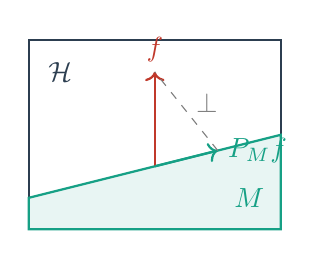
\begin{tikzpicture}[scale=0.8]
        % 希尔伯特空间 H
        \draw[thick, headerblue] (-2, -1) rectangle (2, 2);
        \node[headerblue] at (-1.5, 1.5) {$\mathcal{H}$};
        
        % 子空间 M
        \draw[thick, section2, fill=section2!10] (-2, -0.5) -- (2, 0.5) -- (2, -1) -- (-2, -1) -- cycle;
        \node[section2] at (1.5, -0.5) {$M$};
        
        % 向量 f
        \draw[->, thick, accentcolor] (0, 0) -- (0, 1.5) node[above] {$f$};
        
        % 投影 P_M f
        \draw[->, thick, section2] (0, 0) -- (1, 0.25) node[right] {$P_M f$};
        
        % 误差 f - P_M f
        \draw[dashed, gray] (1, 0.25) -- (0, 1.5);
        \node[right, gray] at (0.5, 1) {$\perp$};
        
    \end{tikzpicture}
    \end{center}

    \hspace{1em}泛函分析把\textbf{函数}看作无穷维向量空间中的\textbf{点}。
    \vspace{4pt}
    
    \subt{三大核心视角}
    \begin{itemize}[itemsep=4pt]
        \item \textbf{完备性 (Completeness)}: 
        为什么我们要用 Lebesgue 积分而不是 Riemann 积分?因为 $L^2$ 空间是完备的 (Hilbert),而 $C[a,b]$ 不是。完备性保证了柯西序列一定有极限 (不会跑出空间外)。
        
        \item \textbf{对偶性 (Duality)}: 
        通过研究作用在物体上的测量 (泛函),来研究物体本身。就像通过投影来重构三维物体。
        
        \item \textbf{紧致性 (Compactness)}: 
        在无穷维空间,有界闭集不一定是紧的 (单位球不紧)。这导致了无穷维分析的种种困难,但也催生了弱拓扑等深刻概念。
    \end{itemize}
    
    \vspace{6pt}
    \centering\textit{\footnotesize 有限维是特例,无穷维才是常态。}
\end{mybox}

\end{multicols*}

\end{document}
